\chapter{Implementação}
\label{sec-implementacao}
Após a definição do escopo \ref{sec:escopo}, do diagrama de classes \ref{sec:diagrama-de-classes}, do design e história do jogo \ref{sec:jogo} das ferramentas que serão utilizadas discutidas no capítulo \ref{sec-referencial}, e uma motivação em mente temos uma base sólida para partir para a implementação. Neste capítulo, são apresentados os detalhes relacionados à implementação do software desenvolvido, bem como algumas das decisões de implementação tomadas com base na seção anterior. O objetivo deste capítulo é fornecer uma visão clara e detalhada de como o software foi estruturado e construído, demonstrando as escolhas técnicas realizadas para atender aos requisitos definidos previamente.

\section{Definições Iniciais}
Antes de começar um jogo \textit{pixel art} é importante definir qual vai ser o tamanho de cada \textit{tile}, os tamanhos mais comuns são 16 x 16, 32 x 32 e 64 x 64, nesse trabalho foi escolhido o tamanho 64 x 64 é importante que todos os tiles presentes no jogo respeitem o mesmo tamanho para uma melhor harmonia visual, e proporções de objetos compatíveis.

\section{Principais Funções}
Nessa seção serão detalhadas as principais funções que garantem o funcionamento adequado do software desenvolvido, a abordagem inclui uma explicação minuciosa sobre os módulos centrais abordando suas finalidades, interações e relevância para o cumprimento dos objetivos do sistema. Além disso, serão discutidas as escolhas realizadas durante o desenvolvimento, evidenciando como essas funções se complementam.

\lstinputlisting[label=lst-main, caption=Main, language=Python, float=htpb]{codigos/main.py}
\clearpage
A primeira coisa a se fazer em um projeto Pygame é inicializa-lo \textit{pygame.init()} isso inicializará todos os módulos do Pygame, com isso feito é possível efetuar algumas configurações iniciais como por exemplo definir um título e redimensionar o tamanho da janela do jogo, esse passo é realizado somente em \textit{home} como mostra a listagem \ref{lst-home} a tela inicial do jogo, aqui na main \ref{lst-main} é apenas feita as chamadas para cada transição, sendo quatro possíveis i) iniciar um novo jogo; ii) abrir a tela de créditos; iii) abrir a tela de controles do jogo e iv) sair do jogo. Para gerenciar essa troca de contexto são criadas três variáveis de controle \textit{home\_open, credits\_open} e \textit{controls\_open} todas do tipo \textit{bool} que servem para definir qual aba estará sendo renderizada, não sendo possível mais de uma delas serem verdadeiras simultaneamente. Também são instanciados três objetos \textit{Home}, \textit{Credits} e \textit{Controls} que são as classes que definem a respectiva tela, a variável de controle \textit{home\_open} é a única inicializada como verdadeiro pois é a tela que será mostrada inicialmente. Esse programa fica em um \textit{loop} enquanto captura os eventos e \textit{inputs} do jogador na tela inicial.
\lstinputlisting[label={lst-home}, caption=Home, language=Python, float=htpb]{codigos/home.py}


Em \textit{home} como mostra a listagem \ref{lst-home} definimos o tamanho da tela 1280 x 720, importamos as imagens e áudios que são usados nessa tela, reproduzimos a musica e criamos uma variável \textit{index}, essa variável é utilizada para saber qual opção o jogador escolheu sendo eles.
\begin{itemize}
    \item \textbf{index 0:} sai do \textit{loop} do menu e inicializa o jogo;
    \item \textbf{index 1:} abre a tela de créditos; 
    \item \textbf{index 2:} abre a tela de controles;
    \item \textbf{index 3:} sai do jogo;
\end{itemize}
Essa troca de contexto é feito a partir das funções de \textit{callback} \textit{run\_game}, \textit{run\_credits}, \textit{run\_game\_controls} nestas que tem a finalidade de alterar as variáveis de controle como mostra a listagem \ref{lst-callback} a seguir. 
\begin{lstlisting}[label= lst-callback,language=Python,breaklines, caption= Função de \textit{callback} responsávél por alterar a variável de controle.]
    def run_credits():
        global credits_open; credits_open = True
        global home_open; home_open = False
\end{lstlisting}

Ainda em \textit{home} para explicar a função \textit{draw\_menu} é necessário explicar alguns conceitos do pygame. Em Pygame tudo que lidamos é baseado em figuras geométricas, ou seja se queremos desenhar uma imagem em um ponto específico, ou queremos posicionar um \textit{sprite} em determinado local, devemos ter um objeto da classe \textit{Rect} para conseguir fazer isso, essa classe também é utilizada para verificar colisões e fazer movimentação de objetos, \textit{Rect} tem os seguintes parâmetros.
\begin{itemize}
    \item \textit{\textbf{x:}} posição em x em que sera desenhado;
    \item \textit{\textbf{y:}} posição em y em que sera desenhado;
    \item \textit{\textbf{width:}} largura do retângulo;
    \item \textit{\textbf{height:}} altura do retângulo;
\end{itemize}

Normalmente não queremos jogar com personagem que seja um retângulo, ou interagir com NPC's (\textit{Non Playable Character}) personagem não jogável em tradução livre que sejam quadrados ou círculos, então associamos uma imagem a esse objeto retângulo, o método \textit{pygame.image.load} carrega uma imagem para o Pygame passando o arquivo como parâmetro e retorna um objeto \textit{Surface} essa classe Surface é utilizada para a representação das imagens no Pygame a figura \ref{fig:player} mostra o resultado da associação de uma imagem a um retângulo.
\begin{figure}[h!]
    \centering
    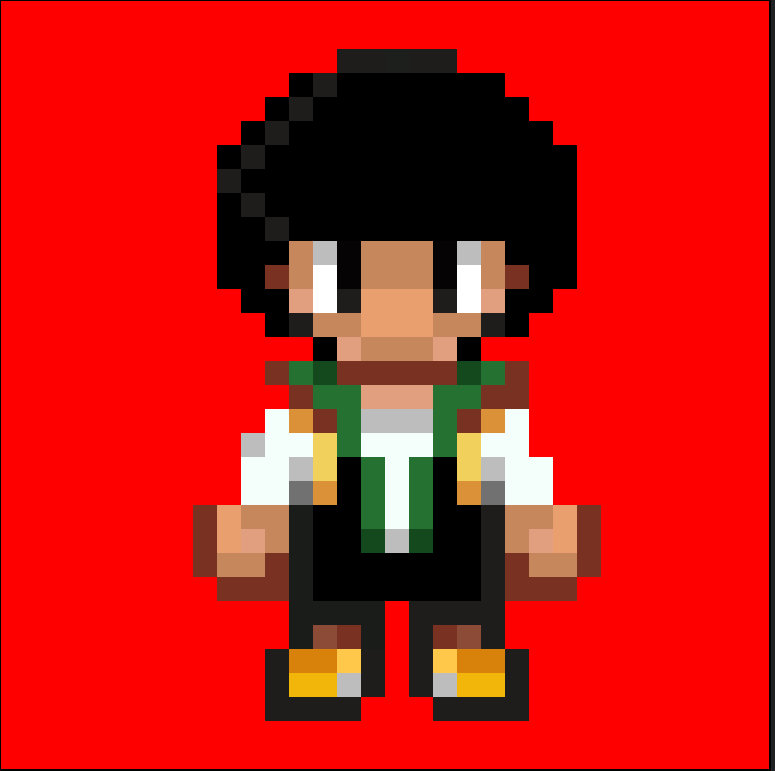
\includegraphics[width=0.5\linewidth]{figuras/player.png}
    \caption{Exemplo de retângulo associado a imagem do personagem principal, a area vermelha representa o retângulo associado ao \textit{player}}
    \label{fig:player}
\end{figure}

\pagebreak
Com essas informações podemos explicar a função \textit{draw\_menu} essa que é responsável por desenhar as informações na tela \textit{home}, a imagem de \textit{background} e os retângulos de seleção, para causar o efeito de iluminação sobre os retângulos ao selecionar cada index é feito o uso do método \textit{blit} do pygame, esse método desenha uma imagem sobre outra imagem, ela tem a seguinte assinatura.
\begin{itemize}
    \item \textit{\textbf{source}:} A imagem \textit{Surface} a ser desenhada sobre o \textit{Surface} atual;
    \item \textit{\textbf{dest (opcional):}} Posição onde será desenhado a imagem, sendo o padrão o canto superior esquerdo (0, 0);
    \item \textit{\textbf{area (opcional):}} A delimitação da área retangular para desenhar;
    \item \textit{\textbf{special\_flags (opcional):}} Controla como as cores do da imagem serão combinadas com a Superfície;
\end{itemize}
É graças ao quarto parâmetro \textit{special\_flags} que é possível causar esse efeito, usando a \textit{flag} \textit{BLEND\_RGB\_ADD } misturamos as cores RGB da mesma imagem com o fundo branco e é adicionado os canais de cor de origem aos canais de cor de destino.

\begin{figure}[h!]
    \centering
    
\includegraphics[width=1\linewidth]{figuras/blit_example.png}
    \caption{Exemplo de sobreposição de imagens com o método \textit{blit}}
    \label{fig:blit-example}
\end{figure}

A operação de \% (resto da divisão) é feita sobre o index para garantir que a opção selecionada pelo jogador seja somente uma das opções definidas, a variável \textit{new\_rect} que tem armazenada um retângulo que será a área a ser desenhada na tela. Todos os retângulos de seleção da tela inicial tem o tamanho fixo 123 x 90, o que muda é a posição que ele sera desenhado, que varia de acordo com o index selecionado, tendo uma verificação para o programa saber qual imagem será desenhada.

\newpage
No Pygame um \textit{sprite} pode ser representado com a classe nativa \textit{Sprite}. Herdar essa classe base e adicionar os atributos e métodos que são do nosso interesse é muito útil, especialmente se usada em conjunto com classe container \textit{Groups}, nela é possível adicionar Sprites que podem ser criados para comportamentos específicos, por exemplo, se queremos criar um grupo de sprites que tenham o comportamento de matar o jogador ao ser colidido poderíamos criar um \textit{Group} chamado \textit{hitkill\_sprites} e adicionar todos os sprites que desejamos que tenha esse comportamento, para realizar a ação de matar o \textit{player} bastaria percorrer \textit{hitkill\_sprites} e verificar a colisão, veja no exemplo da listagem \ref{lst:hitkill-sprite}
\lstinputlisting[label=lst:hitkill-sprite, caption=\textit{Hitkill Sprites}, language=Python, float=htpb]{codigos/hitkill_sprites.py}
\lstinputlisting[label=lst:game, caption=Classe \textit{Game}, language=Python, float=htpb]{codigos/game.py}



Em nosso caso fazemos o uso desse recurso na classe \textit{Game} a seguir na listagem \ref{lst:game}, no Super Labes World temos cinco possíveis comportamentos para os sprites podendo um \textit{sprite} pertencer a mais de um grupo, sendo eles:
\begin{itemize}
    \item \textit{\textbf{collision\_sprites: }}Variável que contém todos os \textit{sprites} colidíveis do jogo no mapa atual;
    \item \textit{\textbf{character\_sprites: }}Variável que contém todos os \textit{sprites} de personagens do game no mapa atual;
    \item \textit{\textbf{transition\_sprites: }}Variável que contém todos os \textit{sprites} de colisão no mapa atual;
    \item \textit{\textbf{dialogs\_sprites: }}Variável que contém todos \textit{sprites} que geram uma caixa de diálogo no mapa atual;
    \item \textit{\textbf{interaction\_sprites: }}Variável que contém todos os \textit{sprites} do jogo que são interativos;
\end{itemize}

A classe \textit{Game} também responsável por inicializar todas as variáveis, \textit{assets} e chamar a função \textit{import\_assets}, essa que carrega para o programa todos os \textit{assets} do jogo será explicada na listagem \ref{lst-import-assets} e chama também o método \textit{setup} listagem \ref{lst-setup} que que carrega e inicializa o mapa inicial.


\lstinputlisting[label=lst-import-assets, caption=Import Assets, language=Python, float=htpb]{codigos/import_assets.py}
\clearpage
O método \textit{import\_assets} da listagem \ref{lst-import-assets} é responsável por fazer a importação e alocação de todos os mapas e assets do jogo. A atribuição desses \textit{assets} é feita através de um dicionário para melhor organização do código sendo as possíveis chaves e valores.


\begin{table}[h!]
	\caption{Especificação dos dicionários de assets.}
	\label{tbl-especificacao-dicionario}
	\centering
	\renewcommand{\arraystretch}{2}
	\begin{small}
		\begin{tabular}{ | p{35mm} | p{35mm} | p{65mm} |}\hline \rowcolor{MidnightBlue}
                \hline
                Dicionário & Chaves & Valores \\
                \hline
                \textit{tmx\_maps} & \textit{map\_name} & Arquivo TMX \\ 
                \hline
                \multirow{3}{4em}{overworld\_frames} 
                & \textit{characters} & \textit{Sprites} de personagems \\ 
                & \textit{water} & \textit{Sprites} de água \\ 
                & \textit{lake} & \textit{Sprites} das bordas do lago \\ 
                \hline
                \multirow{3}{4em}{fonts} 
                & \textit{dialog} & fonte do diálogo \\ 
                & \textit{bold} & Fonte negrito \\ 
                & \textit{regular} & Fonte do inventário e computador \\ 
                & \textit{regular\_mid} & Fonte igual a anterior com tamanho 22 \\ 
                & \textit{regular\_big} & Fonte igual a anterior com tamanho 34 \\ 
                \hline
                \multirow{3}{4em}{interface\_frames} 
                & \textit{interface} & \textit{Sprites} com os \textit{layouts} da interface \\ 
                & \textit{items} & \textit{Sprites} com os items do inventario \\ 
                & \textit{interactive\_objects} & \textit{Sprites} que tem algum tipo de animação ao interagir \\ 
                \hline

                \end{tabular}
	\end{small}
\end{table}

\clearpage
\lstinputlisting[label=lst-setup, caption=Setup, language=Python, float=htpb]{codigos/setup.py}
\clearpage
O método a anterior \textit{setup} ilustrado na listagem \ref{lst-setup} é responsável por carregar o mapa e iniciar todos os \textit{sprites} presentes no mapa passado como argumento, para isso é necessário antes limpar os \textit{sprites} do mapa anterior, essa etapa é importante para limpar os sprites do mapa anterior após uma transição, após isso é feito uma série de \textit{loops} sobre todas as camadas presentes no mapa \textit{.tmx} criado no \textit{tiled}, nesse loop é feita a associação de cada \textit{sprite} com os seus respectivos grupos, sendo eles.
\begin{table}[h!]
	\caption{Tabela especificando os tipos de \textit{sprites} presentes em Super Labes World}
	\label{tbl-especificacao-sprites}
	\centering
	\renewcommand{\arraystretch}{3}
	\begin{small}
		\begin{tabular}{ | p{37mm} | p{23mm}  | p{52mm} | p{30mm} | }\hline \rowcolor{MidnightBlue}
			\centering{\textbf{Classe}} & \centering{\textbf{Camadas}} & \textbf{Descrição} & \textbf{Grupos} \\\hline		
                \centering{\textit{Sprite}} & \centering{\textit{Terrain, Terrain Top, Terrain Objects}} & {Classe com os tiles da camada mais baixa sem colisões} & {\textit{all\_sprites}} \\\hline
                \centering{\textit{AnimatedSprite}} & \centering{\textit{Lake, Lake Edges}} & {Classe com tiles animados do lago sem colisão} & {\textit{all\_sprites}} \\\hline			
                \centering{\textit{CollidableSprite}} & \centering{\textit{Objects}} & {Classe com os sprites de objetos do jogo com colisão} & {\textit{all\_sprites, collision\_sprites}} \\\hline		
                \centering{\textit{InteractiveSprite}} & \centering{\textit{Interactive Objects}} & {Classe com os sprites com interação com colisão} & {\textit{all\_sprites, collision\_sprites, interactive\_sprites}} \\\hline	
                \centering{\textit{CollisionSprite}} & \centering{\textit{Collisions}} & {Classe com as colisões sem uma imagem} & {\textit{collision\_sprites}} \\\hline		
                \centering{\textit{CollidableDialogSprite}} & \centering{\textit{Dialogs}} & {Classe com os sprites de diálogo} & {\textit{dialog\_sprites}} \\\hline		
                \centering{\textit{TransitionSprite}} & \centering{\textit{Transitions}} & {Classe que armazena os sprites de transição sem imagem} & {\textit{transition\_sprites}} \\\hline		
                \centering{\textit{Player}} & \centering{\textit{Entities}} & {Classe do jogador principal} & {\textit{all\_sprites}} \\\hline		
                \centering{\textit{Character}} & \centering{\textit{Entities}} & {Classe para representar as entidades de personagens do jogo} & {\textit{all\_sprites, collision\_sprites, characters\_sprites}} \\\hline		
		\end{tabular}
	\end{small}
\end{table}
\clearpage
\section{Personagens}
Os personagens de um jogo são uma peça fundamental especialmente paga um jogo do gênero RPG, eles desempenham um papel central na construção da experiência narrativa e interativa e enriquecem fortemente a ambientação do jogo, esse capítulo vai abordar em mais detalhes como foi feita a criação de personagens

Os sprites de personagens do jogo são basicamente imagens no formato png (Portable Network Graphics), desenhados no programa aseprite \ref{fig:aseprite} cada uma com o tamanho 512 x 512, no jogo essa imagem é subdividida em 16 quadrados iguais de tamanho 128 x 128 como mostra a figura \ref{fig:player-animation}
Os personagens são adicionados pelo ferramenta Tiled citado na seção \ref{sec:tiled} para carregar os personagens do jogo um recurso do software chamado \textit{Insert Point}, pontos são os objetos mais simples que é possível colocar em um mapa. Eles representam apenas uma localização e não podem ser redimensionados ou girados mas é possível adicionar metadados que serão usados para a identificação de cada personagem, as propriedades inseridas são.
\begin{itemize}
    \item \textbf{\textit{character\_id: }}É com essa variável que lidamos para definir qual dos sprites será mostrado nesse personagem ;
    \item \textbf{\textit{direction: }}Define qual é a posição inicial do jogador ;
    \item \textbf{\textit{pos: }}Mapa anterior que o player estava antes da transição, é necessário por que todo mapa tem pelo menos dois \textit{players} devido a transição de ida e de volta essa variável então é usada para o Pygame saber qual das posições desenhar o jogador ;
\end{itemize}

\begin{figure}[h!]
    \centering
    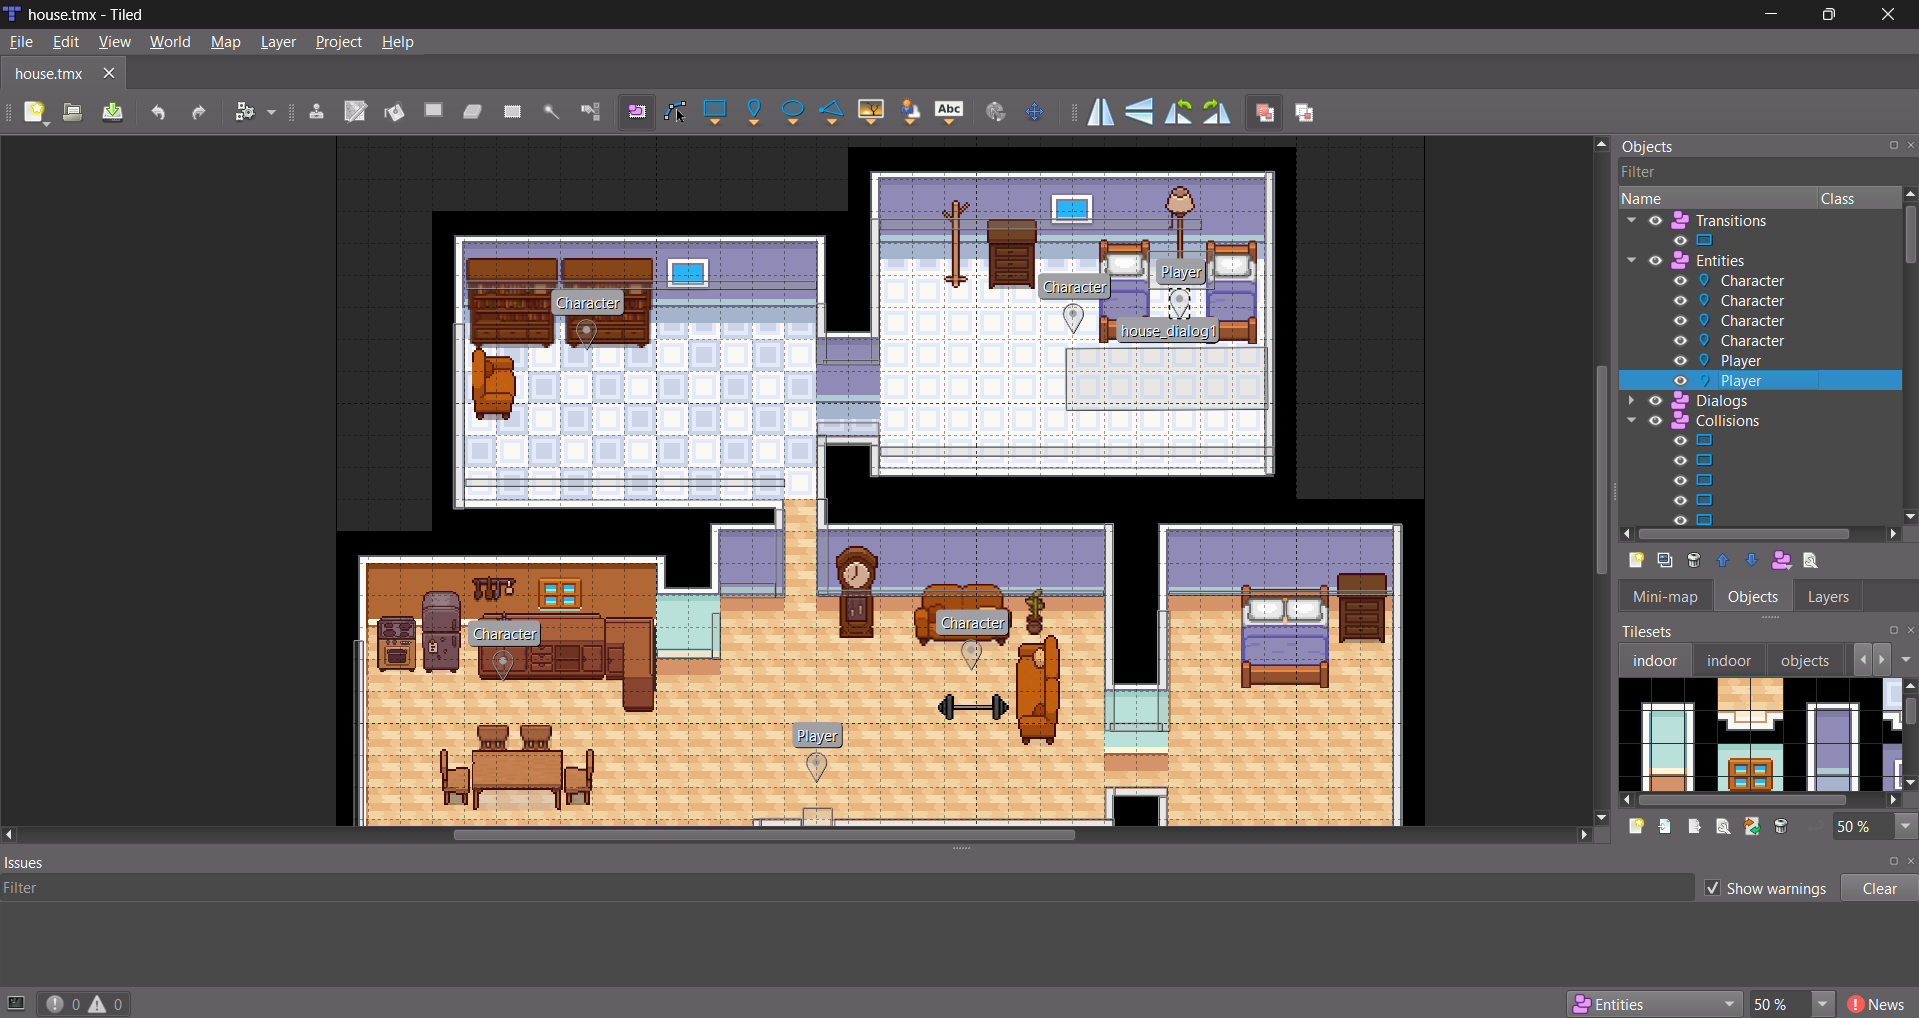
\includegraphics[width=1\linewidth]{figuras/tiled-house.png}
    \caption{Posicionamento de Objetos no Software Tiled }
    \label{fig:tiled-house}
\end{figure}

\begin{figure}[h!]
    \centering
    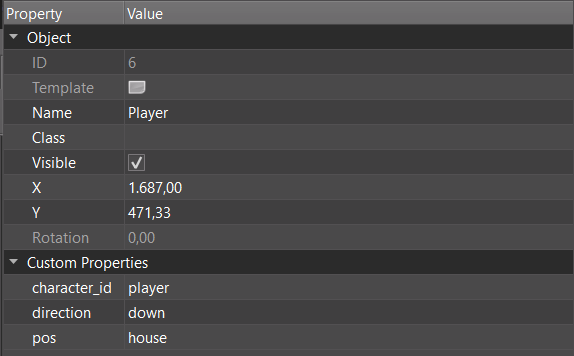
\includegraphics[width=1\linewidth]{figuras/tiled-player-properties.png}
    \caption{Propriedades da Entidade Player no Tiled}
    \label{fig:tiled-player-propertiesl}
\end{figure}

\clearpage
A Animação como explicado na seção \ref{sec:animacao} é uma ilusão gerada pela sequência de imagens sendo alternadas a uma determinada velocidade,  no Super Labes World, é feito o uso dessa técnica, a partir de um dicionário, sendo a chave o nome da posição em que o jogador se encontra e os valores são as imagens que representam essa posição como mostra a figura a seguir:
\begin{enumerate}
    \item \textit{\textbf{down:}} contém as imagens 1, 2, 3 e 4;
    \item \textit{\textbf{down\_idle:}} imagem 1;
    \item \textit{\textbf{left:}} contém as imagens 5, 6, 7 e 8;
    \item \textit{\textbf{left\_idle:}} contém a imagem 5;
    \item \textit{\textbf{right:}contém as imagens 9, 10, 11 e 12};
    \item \textit{\textbf{right\_idle:}} contém a imagem 9;
    \item \textit{\textbf{up:}} contém as imagens 13, 14, 15 e 16 ;
    \item \textit{\textbf{up\_idle:}} contém a imagem 13;
\end{enumerate}
\begin{figure}[h!]
    \centering
    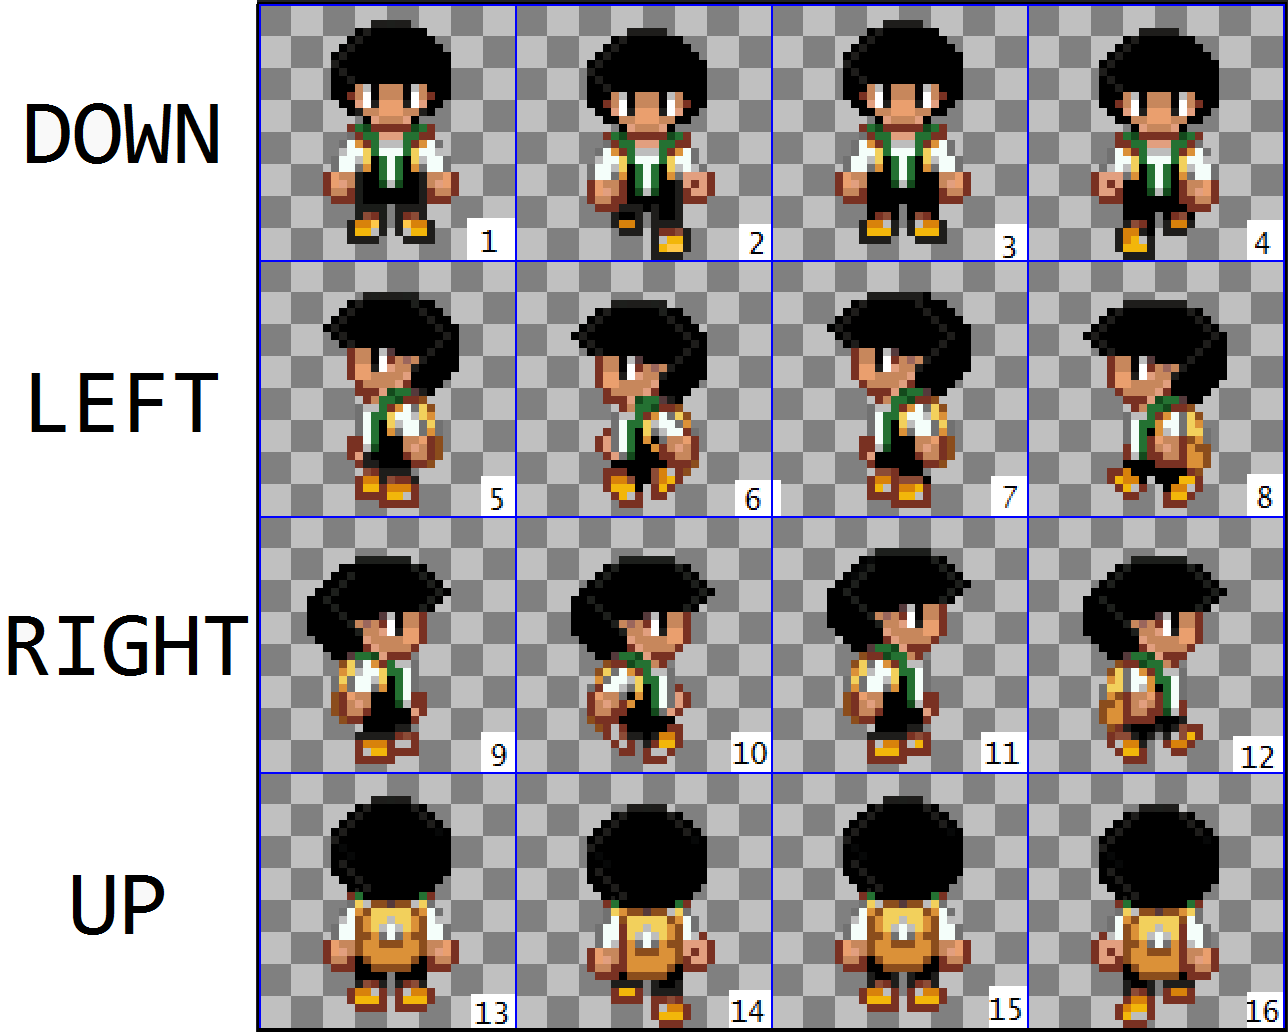
\includegraphics[width=0.5\linewidth]{figuras/player-animation.png}
    \caption{\textit{Sprite} de Animação do \textit{Player} }
    \label{fig:player-animation}
\end{figure}

% detalhar mais aqui
Para realizar a animação do personagem principal no código, é necessário algumas funções
uma função que fique intercalando os frames de acordo com o estado atual do jogador
uma função que retorne o estado atual do jogador
uma função para capturar a entrada de dados do jogador e retorne um vetor com a direção
uma função para movimentação
e uma função para atualização;

\lstinputlisting[label=lst-player-animation, caption=Player animation, language=Python, float=htpb]{codigos/player_animation.py}

\clearpage
Na figura \ref{fig:player} existe um problema, o retângulo do player é muito maior do que a imagem do personagem, existe um método do Pygame para lidar com isso  \textit{inflate} essa função diminui o tamanho de um retângulo se passado um valor negativo e aumenta caso positivo, a listagem \ref{lst-player-hitbox} mostra a utilização do método e a figura \ref{fig:player-hitbox} simula o resultado diminuindo a largura pela metade e 60 píxels de altura.

\begin{lstlisting}[language=Python,breaklines, caption= Uso da Função \textit{inflate}, label= lst-player-hitbox]
self.hitbox = self.rect.inflate(-self.rect.width / 2, -60)
\end{lstlisting}
\begin{figure}[h!]
    \centering
    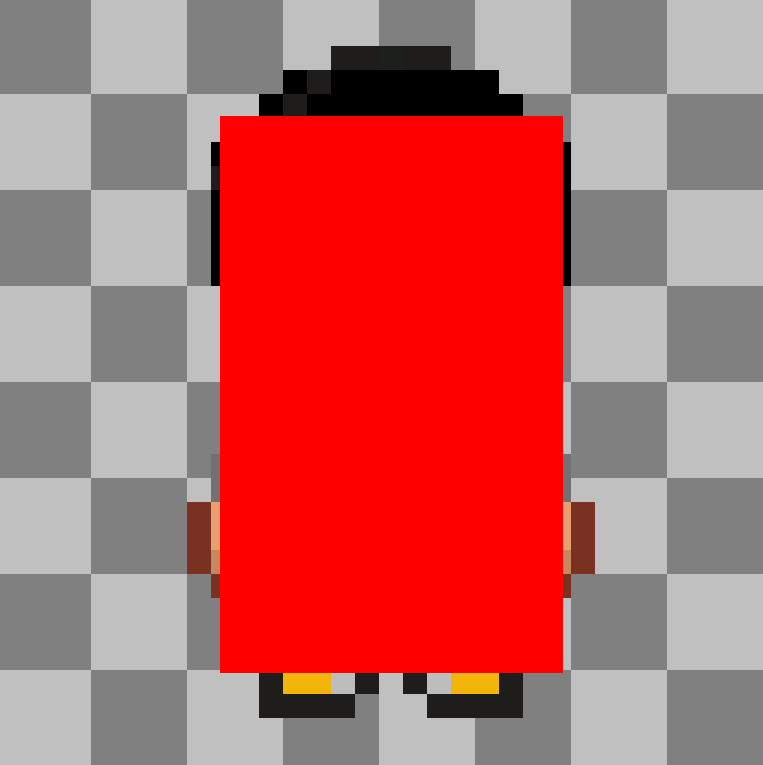
\includegraphics[width=0.5\linewidth]{figuras/player-hitbox.png}
    \caption{\textit{Hitbox} do Personagem Principal após o a Chamada do Método \textit{blit}}
    \label{fig:player-hitbox}
\end{figure}






\section{Game Loop do Super Labes World}
\label{sec:game-loop-super-labes-world}
% game loop
\lstinputlisting[label=lst-game-loop, caption=Main, language=Python, float=htpb]{codigos/game_loop.py}
\newpage
O game loop é o núcleo principal do jogo , ele é responsável por manter o jogo em execução contínua, nele são processados um conjunto tarefas continuamente, no nosso programa, a função é a ilustrada na listagem \ref{lst-game-loop}, o loop e composto pelos seguintes passos.
\begin{enumerate}
    \item Preencher o \textit{background} de preto;
    \item Atualizar o valor do \textit{delta time} explicado na seção \ref{sec:delta-time}
    \item Verificar o evento de fechar o jogo;
    \item Detectar e lidar a entrada de teclado do jogador
    \item Verificar se o jogador colidiu com um \textit{sprite} de transição quando for o caso chama a função \textit{setup} com os parâmetros do mapa a ser transicionado;
    \item Verificar se o jogador colidiu com alguma caixa de diálogo, se sim então chamando a função para criar o diálogo com a mensagem;
    \item Atualizar todos os sprites da tela; 
    \item Desenhar todos os sprites da tela;
    \item Verificar se tem alguma sobreposição do jogo, sendo elas;
        \begin{itemize}
        \item \textit{\textbf{dialog\_open: }} verdadeiro quando o jogador aperta \textit{"backspace"} 
        próximo a uma personagem do jogo, então troca de contexto do \textit{loop} principal para o \textit{loop} da classe \textit{Dialog};
        \item \textit{\textbf{inventory\_open: }}verdadeiro caso de o jogador aperte a tecla "i", troca o contexto do \textit{loop} principal para o \textit{loop} da classe \textit{Inventory}; 
        \item \textit{\textbf{computer\_open: }} verdadeiro quando o jogador aperta "\textit{backspace}" próximo a \textit{InteractiveObject} com o \textit{"item\_id"} = \textit{computer}, troca de contexto do \textit{loop} principal para o \textit{loop} da classe \textit{Computer};
        \item \textit{\textbf{battle\_open: }}  verdadeiro quando o jogador o jogador responde sim para um desafio de um personagem com questões, nesse caso troca-se de contexto para a batalha;
        \item \textit{\textbf{choose\_dialog\_open: }} verdadeiro ao fim de um diálogo de um personagem que contém questões e que não foi derrotado;
    \end{itemize}
\end{enumerate}
% input
A função \textit{input} é a responsável por detectar e lidar com todas as entradas de comandos do jogador, nela são definidas todos os possíveis comandos e controles do jogo. É importante adicionar variáveis de controle afim de não permitir que o jogador se movimente enquanto estiver dialogando com um personagem,  por isso antes de verificar a entrada do jogador é conferido os valores das variáveis \textit{booleanas} \textit{dialog\_open} que se verdadeira o jogador está dialogando, \textit{choose\_dialog\_open} se verdadeiro o jogador está na interface de seleção da resposta e \textit{battle\_open} verdadeira quando o jogador está em uma batalha. Se falso para as três variáveis então é examinado qual tecla o jogador aperta sendo as possíveis.
\begin{itemize}
    \item \textbf{Tecla I: }abre o inventário e coloca o player no estado bloqueado;
    \item \textbf{Tecla ESC: }fecha as interfaces de inventário, computador e tira o jogador do estado bloqueado;
    \item \textbf{Tecla \textit{Backspace}: }a tecla de interação do jogador, quando pressionada é necessário verificar se o jogador está perto a um personagem, ou a um objeto interativo quando for o caso a função leva para o respectivo tratamento;
\end{itemize}

Veja a seguir na listagem \ref{lst-input} o código especificamente.
\lstinputlisting[label=lst-input, caption=Input, language=Python, float=htpb]{codigos/input.py} 







